\documentclass[runningheads,a4paper]{llncs}

\usepackage[latin1]{inputenc}
\usepackage{graphicx,color,url}
\usepackage[dvips]{epsfig}
\usepackage{verbatim}
\usepackage{tikz}
\usetikzlibrary{shapes,arrows}
\usetikzlibrary{calc,patterns,snakes,decorations.pathmorphing,decorations.markings}
\usetikzlibrary{positioning}
\usepackage{amsmath}

\usepackage{tabularx} % better tables
\usepackage{float}
\setlength{\extrarowheight}{3pt} % increase table row height
\newcommand{\tableheadline}[1]{\multicolumn{1}{c}{\spacedlowsmallcaps{#1}}}
\newcommand{\myfloatalign}{\centering} % to be used with each float for alignment
\usepackage{caption}
\captionsetup{font=small} % format=hang,
\usepackage{subfig}
\usepackage[ruled]{algorithm2e}
%\providecommand{\tabularnewline}{\\}
\usepackage{listings}
\usepackage{color}
\usepackage{graphicx}
\newcommand{\keywords}[1]{\par\addvspace\baselineskip
	\noindent\keywordname\enspace\ignorespaces#1}

\definecolor{dkgreen}{rgb}{0,0.6,0}
\definecolor{gray}{rgb}{0.5,0.5,0.5}
\definecolor{mauve}{rgb}{0.58,0,0.82}
\definecolor{gray}{rgb}{0.4,0.4,0.4}
\definecolor{darkblue}{rgb}{0.0,0.0,0.6}
\definecolor{lightblue}{rgb}{0.0,0.0,0.9}
\definecolor{cyan}{rgb}{0.0,0.6,0.6}
\definecolor{darkred}{rgb}{0.6,0.0,0.0}


\lstset{
	basicstyle=\ttfamily\footnotesize,
	columns=fullflexible,
	showstringspaces=false,
	numbers=left,                   % where to put the line-numbers
	numberstyle=\tiny\color{gray},  % the style that is used for the line-numbers
	stepnumber=1,
	numbersep=5pt,                  % how far the line-numbers are from the code
	backgroundcolor=\color{white},      % choose the background color. You must add \usepackage{color}
	showspaces=false,               % show spaces adding particular underscores
	showstringspaces=false,         % underline spaces within strings
	showtabs=false,                 % show tabs within strings adding particular underscores
	frame=none,                   % adds a frame around the code
	rulecolor=\color{black},        % if not set, the frame-color may be changed on line-breaks within not-black text (e.g. commens (green here))
	tabsize=2,                      % sets default tabsize to 2 spaces
	captionpos=b,                   % sets the caption-position to bottom
	breaklines=true,                % sets automatic line breaking
	breakatwhitespace=false,        % sets if automatic breaks should only happen at whitespace
	title=\lstname,                   % show the filename of files included with \lstinputlisting;
	% also try caption instead of title  
	commentstyle=\color{gray}\upshape
}


\lstdefinelanguage{XML}
{
	morestring=[s][\color{mauve}]{"}{"},
	morestring=[s][\color{black}]{>}{<},
	morecomment=[s]{<?}{?>},
	morecomment=[s][\color{dkgreen}]{<!--}{-->},
	stringstyle=\color{black},
	identifierstyle=\color{lightblue},
	keywordstyle=\color{red},
	morekeywords={material, minWidth, maxWidth, width, rotation, type, id, x, y, source, target, version}% list your attributes here
}

\begin{document}

\mainmatter  % start of an individual contribution

% first the title is needed
\title{Free Form Evolution for Angry Birds Level Generation}
% Antonio - I fix the format of the title and the name of the game

% a short form should be given in case it is too long for the running head
\titlerunning{}

% the name(s) of the author(s) follow(s) next
%
% NB: Chinese authors should write their first names(s) in front of
% their surnames. This ensures that the names appear correctly in
% the running heads and the author index.
%

\author{A. N. Onymous\inst{1}%
\thanks{No Institute}}
\authorrunning{Anonymous, A}
% (feature abused for this document to repeat the title also on left hand pages)

% the affiliations are given next; don't give your e-mail address
% unless you accept that it will be published
%\institute{Dept. of Computer Architecture and Technology, University of Granada, Spain}
\institute{Anonymous Institute}


%
% NB: a more complex sample for affiliations and the mapping to the
% corresponding authors can be found in the file "llncs.dem"
% (search for the string "\mainmatter" where a contribution starts).
% "llncs.dem" accompanies the document class "llncs.cls".
%

\maketitle

%
%%%%%%%%%%%%%%%%%%%%%%%%%%%%%%%   ABSTRACT   %%%%%%%%%%%%%%%%%%%%%%%%%%%%%%%
%
\begin{abstract}
This paper presents an approach for building stable structures under gravity 
for the physics-based puzzle game Angry Birds. Thus, a search-based procedural 
level generation method has been developed using evolutionary algorithms. 
Different representations and operators have been considered and studied. In 
order to evaluate the stability of the levels, they are executed in an 
adaptation of an open source version of the game called \textit{Science Birds}. 
% Antonio - abstract do not include references.  ;)
In the same way, an open source evolutionary computation framework has been implemented to fit the requirements of the problem. In order to test the method four experiments have been carried out, obtaining a variety of stable structures.
% Antonio - Speak about the structures and their utility, fun, player's opinion, etc, which are the objectives in PCGs

\keywords{Search-Based Procedural Content Generator, Evolutionary algorithm, 
Game development, Angry Birds, Level generation}
\end{abstract}

%
%%%%%%%%%%%%%%%%%%%%%%%%%%%%%%%   INTRODUCTION   %%%%%%%%%%%%%%%%%%%%%%%%%%%%%%%
%
\section{Introduction}
\label{sec:intro}

%************************************************

% It's probably the best to eliminate subsections. It saves space, and it's a 
%short paper anyway - JJ


%The definition of Procedural Content Generation (PCG) has been
%broadly discussed but there is no agreement. We have plenty of
%examples of what \textit{is} and what \textit{is not} PCG, but every
%definition struggles to cover all cases, either being too inclusive
%or too exclusive. The one we choose here balances well between the
%two, defining

For the purpose of this paper, we define Procedural Game Generation
(PCG) as \textit{the algorithmical creation of game content with
  limited or indirect user input}. 
%Although PCG often uses Artificial Intelligence (AI) techniques, this
%definition does not include all uses of it in games. We do not
%consider Non Playable Character (NPC) behaviour or AI playing agents
%as content, thus they are not PCG either.
Aesthetic elements, game rules, levels, items, stories and characters
among others are considered content in this definition  
\cite{togelius2011procedural}. % If this
                                % definition is not totally yours, you
                                % should give a reference for it.
                                % It is from the same  
                                %\cite{togelius2011procedural}
Note that neither computers nor video games are mentioned in the
definition. In fact, PCG has its roots in analogical games.
%This may
%conflict with the \textit{limited or indirect user input}, but it is
%reasonable to assume that following a detailed set of
%instructions---even if it is done by a human---is not
%\textit{input}.
The underlying concepts used by games such as \textit{Dungeon \& Dragons} still 
prevail in modern video games. \cite{smith2015analog} 
% Using an
%algorithm to assemble pre-designed pieces is a common technique in
%tabletop roleplaying guides---where the algorithm usually consists in
%several dice rolls---such as \textit{Dungeon \& Dragons}.
% It is not
%surprising that one of the early adaptations of PCG to digital
%platforms aimed to generate monsters and dungeons for physical
%games.

There are many PCG methods and it is necessary to look at some traits that 
characterize and differentiate them from each 
other\cite{togelius2016introduction}. The method proposed in this paper is 
described as \textit{offline} ---the PCG occurs before the game session or 
during development---, \textit{necessary} ---the generated content is part of 
the essential structure of the game---, \textit{generic} ---it does not take 
into account player behaviour---, \textit{stochastic} ---it will not produce 
the same output given the same input---, \textit{generate-and-test} ---it 
produces potentially correct solutions that are tested and adjusted in each 
iteration before giving the actual output--- and potentially be either 
\textit{automatic}---where the designer does not take part on the process--- or 
\textit{mixed authorship}, where the generated content is used as a base or 
part of an interactive tool. 

A special kind of \textit{generate-and-test} approach to PCG is
Search-based Procedural Content Generation (SBPCG), which is
usually---but not always---tackled with Evolutionary Algorithms. The
problems faced by SBPCG are not very far from those encountered in
Evolutionary problems.  

The test function grades how good a valid solution is. This is often called 
\textit{fitness function}. In SBPCG, how to evaluate the quality of a solution 
has no straightforward answer. It requires formalizing as a \textit{fitness 
function} how much fun, exciting or engaging certain content is, which are 
usually based in tricky assumptions.

There are three main classes of \textit{fitness functions} in SBPCG\cite{togelius2010search}:

\begin{itemize}
	\item \textit{Direct Fitness Function} where certain easily measurable 
	features are extracted from the generated content and mapped to a 
	fitness value.
	\item \textit{Simulation-Based Fitness Function} where the 
	fitness is calculated using features from an agent's gameplay. 
	\item \textit{Interactive Fitness Function} where the fitness value is 
	obtained from the player, whether it be explicitly or 
	implicitly. 
\end{itemize}

% I've shorten the first part of this section, but I don't know if we better just remove it or remove why replayability, adptative contet and assistance tools are interesting for saving resources. Is there need to define PCG in depth in the previous section then? - Laura
% No, really no need. It's a games track, probably people already know what it is. A general definition and focusing on the specific type we are using is more than enough. - JJ
% OK, it does look good now. No need to eliminate - JJ

The fast pace at which the game industry grows poses a challenge to developers. 
How do we create a vast amount of content that suits 
players' expectations with lower investment? PCG can tackle this by  
increasing replayability, offering adaptative content or reducing designers' 
workload.\cite{togelius2016introduction}


Replayability relies on how interesting is 
playing a game more than once. For designers, this means their 
product offers more with less manually crafted content. 
Games can also engage players by adapting gameplay elements to each individual 
player. The most common way is 
to present users with options to adjust game elements, but with PCG techniques, 
the game itself can change based on in-game player behaviour.
PCG can be used as a tool to assist developers. It can suggest what might be a 
base for later development, enhancing human creativity rather than displacing 
it. 

It is common for AI researchers to turn to games in general as a testing 
environment for AI techniques.
%Some of the earliest problems that AI attempted 
%to solve were checkers and chess in the 50s, even before AI was defined and 
%recognized as a field in the Dartmouth workshop in 1956 
%\cite{nilsson1998artificial}.
This interest in games ---both video games and bard games--- is not 
surprising since they have a rather simple set of rules, they can be a 
challenging task even for a human brain and they offer a wide range of dynamic 
and competitive elements that resemble real-world problems to some extent. The 
interest works in both ways. Many video games use AI techniques to deliver 
better experiences, mainly involving NPC behaviour and PCG.

% These two paragraphs should probably be synthesized to a single
% sentence. - JJ
Having this relationship between academia and industry in mind, the IEEE 
Conference on Computational Intelligence and Games was created\cite{ieee-cig}. 
In 2018, most proposed competitions were centred around playing AI agents for 
specific games or genres, but we can find an exception in the \textit{3rd Angry 
Birds Level Generation Competition}. Participants must build computer programs 
that are able to generate levels for the \textit{Angry Birds} game.
It is a mobile game by Finnish company Rovio Entertainment 
Corporation\cite{angry-birds}, first launched in 2009. 
%The game was a huge success in the \textit{AppStore}
%---being the most downloaded mobile game in 
%history. Having been ported to several other platforms since, it has an 
%animated movie and way too many \textit{spin offs}---around seventeen.
In the game, there is a variety of defensive structures made out of blocks 
and the player has to fire birds from a slingshot
%---apparently they never learnt to fly---
so the structure is destabilized.
What is interesting to us is how heavily the 
game relies in gravity to create interesting puzzles. The main challenge from 
the PCG perspective is to build stable structures that are robust enough to 
take more than a single shot before crumbling to the ground.

% The main challenge [from the PCG perspective (or similar)] is to build stable 
%structures.. - Mario


The ultimate objective of this project is to build a program capable of 
creating levels for \textit{Angry Birds}. We can break it down to the 
following, more concise, objectives:

\begin{itemize}
	\item Explore the expressiveness and variability of SBPCG using 
	EAs.
	\item Adapt the game code to extract data from execution to 
	evaluate the levels.
	% Adapt the [game code], to extract (readers may think about the actual 
	%game) - Mario 
	\item Produce stable structures under gravity.
	\item Place other elements on the structures to complete the levels.
\end{itemize} 

% Antonio - In my opinion the introduction is extremely long. It should be reduced, doing it more concise, focused on the paper objectives and with a firm motivation based on the existing gap of the state of the art.
 

%The rest of this paper is organized as follows:
%The next section presents the state of the art and related works, and comments their differences with regard to this study, along with its contribution to advance in this research line. TORCS simulator is described in Section \ref{sec:torcs}.
%The proposed fuzzy controller (and its sub-controllers) is detailed in Section \ref{sec:fuzzy_controller}, whereas it is tested in `real' (simulated) races in Section \ref{sec:results}. Obtained results are analyzed and compared 
%with other controllers are given in the same section. Finally, the conclusions and future lines of work are included in Section \ref{sec:conclusions}.


%%%%%%%%%%%%%%%%%%%%%%%%%%%%%%  STATE OF THE ART  %%%%%%%%%%%%%%%%%%%%%%%%%%%%%%
\section{Background and State of the Art}
\label{sec:soa}

% Antonio - TODO: Introduce the PCG in similar games

PCG is becoming more frequently used in new games as one of the main tools for supporting designers and developers. It has a growing relevance which has been also translated into the arising of new international competitions aimed to design algorithms to generate interesting/funny/enjoyable contents for different games, such as Super Mario (a clone of it) \cite{MarioAI_Level_12}, not specified General Video Games \cite{GAIG_LevelGeneration_18,Khalifa_GVGLG_16}, or recently, for Angry Birds \cite{AngryBirds_LevelGeneration_18}.


% -------- Antonio ---- TO BE CONTINUED --------------------


The main contributions related wit this paper objectives are entries presented to previous editions of the Angry Birds Level Generation Competition. 
From them, we could extract two main approaches to the problem that stand out: constructive and search-based.

% Introduce the two types, once subsections have been eliminated - JJ

In the two solutions proposed by Matthew Stephenson and Jochen Renz \cite{stephenson2017generating} \cite{stephenson2016procedural} the structures displayed on the level are constructed from the top down, in several phases. 

First, they build a structure recursively, each row composed of a single type of block (with a fixed rotation). The likelihood of selecting a certain block is given by a probability table. Then, the blocks are placed using a tree structure, where the first selected block is the peak and blocks underneath it are split into subsets that support the previous row with one, two or three blocks. This ensures local stability, but not global stability, which is tested once the whole structure is completed. The second solution also tries to add variety by replacing some blocks with others of the same height.

After that, other objects (pigs and TNT) are placed. Potential positions for those objects are recorded, first trying to place them in the centre of each block, then right above the edges of it, checking if there is enough space. Available positions are ranked based on structural protection, dispersion, etc. and then filled with the desired number of objects.

The second solution also selects material---which can be stone, ice or wood---based on trajectory analysis, clustering, row grouping, structure grouping or randomly. Weak points are set to stone material and the rest using one of the previous strategies. Trajectory analysis-based strategy sets to the same material all blocks in the trajectory of a shot aimed at a particular pig. Clustering strategy takes a random block, sets its material and propagates to the surrounding blocks that have not been assigned yet. Row grouping and structure blocking apply the same material to a whole row or structure respectively.

Materials also determine which kind of birds will be used in the level, since 
some birds are more efficient against certain materials than others. The number 
of birds available for the player to solve the level is estimated using AI 
agents designed for a different competition. If the AI agents are unable to 
solve the level, it is discarded. The lowest number of birds used by the agents 
is the chosen for the level.

The probability table was tuned using search-based optimization methods.

Following the search-based approach, Lucas Ferreira and Claudio 
Toledo\cite{ferreira2014search} have presented a solution based on SBPCG using 
a genetic algorithm and a game clone developed in Unity Engine to evaluate the 
levels. 

In the genetic algorithm individuals correspond to levels, each represented by 
an array of columns. Each column is a sequence of blocks, pigs and predefined 
compound blocks, using an identification integer. This representation also 
includes the distances between different columns.

The population is initialized randomly following a probability table which 
defines the likelihood of a certain element being placed in a certain position 
inside a column.

For the evaluation, levels are executed in the game which stores data about the 
simulation. The fitness function is described as:

$$ f_{ind} = \frac{1}{3}(\frac{1}{n} 
\sum_{n-1}^{i=0}{v_i}+\frac{\sqrt{(|b|-B)^2}}{Max_b-B}+ \frac{1}{1-|p|})$$ 

where $v_i$ is the average magnitude of the velocity vector for block $i$, 
$|b|$ is the total of blocks in the level and $|p|$ the count of pigs. The rest 
are parameters: $B$ the desired amount of blocks and $Max_b$ the maximum number 
of elements.

The recombination process uses an Uniform Crossover where the new individual is 
generated picking for each position a column from one of the parents which 
occupies the same position. When the parents are not the same length, the 
remaining columns are selected with a $50\%$ of probability. Mutation simply 
changes with a certain probability each element of the individual randomly 
(either being a column element or the distance between columns).

% If possible, add more entries about evolution of free-form structures, which was after all the motivation for this particular algorithm - JJ
% In general or from the competition? - Laura
% In general. The state of the art has to reflect what other people are doing in general - JJ

%%%%%%%%%%%%%%%%%%%%%%%%%%%%  PROBLEM DESCRIPTION  %%%%%%%%%%%%%%%%%%%%%%%%%%%%
\section{Problem Description}
\label{sec:torcs}
% It's probably better if this subsection is eliminated and
% substituted by a reference to the fact that some changes were made
% and that these changes are available. In general, implementation
% details (and code snippets) are not suitable for this kind of
% conferences - JJ


% \subsection{Open Source Simulator}
% \textit{Angry Birds} is not open source software and so the code is not available. As a part of their solution, Lucas Ferreira and Claudio Toledo\cite{ferreira2014search} developed an open source simulation for the game. Since that implementation is available on Github\cite{sciencebirds}, it will be used as a starting point for this part of project. The modified version is available on Github\cite{sciencebirds-adapt} and described in section \ref{ch:gameApdaptation}.

% The game is implemented using the Unity Engine and its code is mainly written in C\#. Levels are not part of the game itself and instead they are parsed from XML files contained in an specific folder in the game hierarchy (which corresponds to the \textit{Assets/StreamingAssets/Levels} directory). Each level is described in a different file, similar to listing \ref{xmlsample}

% \bigskip

% \lstset{language=XML}
% \begin{lstlisting}[caption=Sample level input to show format, label=xmlsample]
% <?xml version="1.0" encoding="utf-16"?>
% <Level width="2">
% <Camera x="0" y="0" minWidth="20" maxWidth="25">
% <Birds>
% <Bird type="BirdRed"/>
% <Bird type="BirdBlack"/>
% </Birds>
% <Slingshot x="-7" y="-2.5">
% <GameObjects>
% <Block type="RectMedium" material="wood" x="2.78" y="-3.18" rotation="0"/>
% <Block type="RectFat" material="wood" x="2.75" y="-2.66" rotation="90.00001"/>
% <Block type="SquareHole" material="stone" x="2.04" y="-2.3" rotation="0"/>
% <Block type="RectSmall" material="wood" x="4.05" y="-3.08" rotation="0"/>
% <Pig type="BasicSmall" material="" x="2.74" y="-1.98" rotation="0"/>
% </GameObjects>
% </Level>
% \end{lstlisting}
% The XML file sets a number of parameters for the level, some of them are key to level generation and others will be ignored by the generator but still needed for the simulation:
% \begin{itemize}
% 	\item Level width 
% 	\item Camera position
% 	\item List of birds, each one with its type (for our objective of making stable structures this will remain constant, although it is important from a game designer's point of view)
% 	\item Slingshot position
% 	\item Game objects list, this one is the most important for level generation. It can contain blocks, pigs or TNT.
% \end{itemize}

% Those elements are then used to build a level, placing the objects in the specified coordinates (note that 0,0 correspond to the centre of the screen, the ground being at $y=-3.5$ in game world units).

% Although the simulation described in \cite{ferreira2014search} does offer an output and it is automated to run through all levels, the implementation provided does not. However, some of these features can be found in the source code.

% \subsection{Modifications to the Open Source Simulator}\label{ch:gameApdaptation}
% Considering the functionality of the existing code, there are a few issues preventing us from using the game as a simulation:

% \begin{itemize}
% 	\item (Issue \#1) Human interaction is needed in order to proceed: there is a main title screen and a level selection. 
% 	\item (Issue \#2) A level will only be finished if the user skips it or if there are no pigs left. If there are no pigs in the level description, the game may have inconsistent behaviour, displaying the \textit{Level cleared} banner or crashing.
% 	\item (Issue \#3) Once a level has been skipped or cleared, data from execution is not stored.
% 	\item (Issue \#4) Skipping the last level results in loading the first level again. 
% \end{itemize}

% It is also worth mentioning that the simulation was intended to run under a Linux distribution. However, this was not possible probably due to issues with the Unity Engine compiler for Linux. Those were presumably fixed in later releases but it is not working on this project, originally created in a much older version although the code itself does not seem to be platform-dependent.

% Modifying the simulation to write data output---Issue \#3--- is fairly simple since the functions were already in the code. However, the data that was being stored was not enough for its purpose. Output XML level was a valid input XML level, which misses some key information about the execution and in this case there was not much interest in obtaining a new valid level. The desired output would look like listing \ref{xmlsampleOUT} (note that encoding was also changed from original): 

% \bigskip

% \lstset{language=XML}
% \begin{lstlisting}[caption=Sample level output to show format, label=xmlsampleOUT]
% <?xml version="1.0" encoding="utf-8"?>
% <Level width="2">
% <Camera x="0" y="0" minWidth="20" maxWidth="25" />
% <Birds>
% <Bird type="BirdRed" />
% </Birds>
% <Slingshot x="-5" y="-2.5" />
% <GameObjects>
% <Block type="RectSmall" material="wood" x="3.78" y="-3.294594" rotation="90" id="0" aVelocity="6.974828E-08" />
% <Block type="SquareTiny" material="wood" x="3.78" y="-2.551131" rotation="90" id="1" aVelocity="1.464643E-07" />
% </GameObjects>
% </Level>
% \end{lstlisting}

% To calculate the average magnitude of velocity for each block, it should be measured at regular time intervals; but, since this and other processes seem to be framerate-dependent, this was achieved by forcing the game to a constant frame rate. Blocks that were destroyed on execution are not present in the output.

% Encoding was changed from \texttt{utf-16} (C\# XML reader/writer default) to \texttt{utf-8} (the only format available for Python's Standard Library XML reader).

% The next logical step is getting rid of interaction. The simulation we are interested in does not require a player (human or AI agent) to play the level since the goal is to know how the level behaves under the game's physics that do not need to---and they do not---match real physics.

% A level will run for a certain amount of time, and then continue to the next one, skipping the main menu and level selection. When the simulation reaches the last level it will end the execution.

% Unity Engine projects are usually divided into scenes. This one has a 
%different scene for the main menu, level selection, loading screen, levels and 
%failure screen. Removing scenes from the screen flow causes side effects such 
%as the first level crashing so instead, the same functions invoked by the GUI 
%are called after initialization takes place in both scenes (main menu and 
%level 
%selection) before the first level. This solves interaction with menus (Issue 
%\#1). 

% In order to skip levels and keeping in mind the velocity of the blocks is already being tracked, the game will load the following scene---the next level---once all blocks reach velocity $0$, which means the blocks have stabilized. Just in case this condition is never met, there is also a time limit of $10s$ for each level (Issue \#2). 

% The remaining issue (Issue \#4) is solved just by checking how many levels have been loaded and the index of the currently playing level.

% I have eliminated the whole subsection above. Some reference to what
% was done here should be inserted elsewhere - JJ

As a part of their solution, Lucas Ferreira and Claudio 
Toledo\cite{ferreira2014search} developed an open source simulation for the 
game. Since that implementation is available on Github\cite{sciencebirds}, it 
will be used as a starting point for this part of the project. The modified 
version is available on Github\cite{sciencebirds-adapt} and the main changes 
revolve around automation and producing output.

%\subsection{Evolutionary Algorithm}\label{ch:Representation}

The most challenging part of the level generation process is to create stable 
structures. As obvious as it is, the main feature of a stable level is that it 
is not in motion. So it seems reasonable to evaluate their stillness as opposed 
to their speed.

$$fitness_{ind} = \frac{1}{|V|}\sum_{i=0}^{b}{V_i} + P_{broken}\cdot(b-|V|)$$

The game output provides the average magnitude of velocity for each block. This 
set is noted as $V$, with $|V|$ being the cardinality of the set. The number of 
blocks in an individual is $b$ and it can differ from the cardinality of $V$ 
since broken blocks are not tracked. The number of broken blocks is $b-|V|$ and 
it is multiplied by a penalization factor, since a level whose blocks break 
without user interaction would not be considered valid. This happens when a 
block free-falls from a certain height or collides with a falling object. 
$P_{broken}$ is set to $100$ since objects in a level do not usually reach that 
velocity, therefore it will separate non-valid levels from potentially good 
ones.

% When we say length of a vector, we think about the norm (the actual lenght) 
% for instance the hypotenuse in a 2D vector. I think here we are talking about 
%the
% number of elements. If V is a set, then the cardinality |V| is right. 
% From your "calculateFitness" this is len so it is a list. 
% I was confused because we are talking about magnitude, velocity, etc. 
% Consider changing the name of V to an ordered set? - Mario
% Done - Laura


Not all levels are evaluated using a simulation, since it is a costly process. 
Although we may know that a given level will perform poorly in the simulation, 
removing it from the population will cause a high loss of diversity. For that 
matter, before testing a level, there are some indicators that a level would 
not be suitable and can be skipped in the simulation. Those are its distance to 
the ground and the number of blocks that overlap.

If the lowest object is not close to the ground is very likely that all blocks 
will break in the impact. Levels that have all their blocks higher than a 
certain threshold will not be simulated in the game. The threshold used is 
$0.1$ in game units and the penalty applied to the fitness value is $10$:
$$f_{distance} = 
\begin{cases}
P_{distance}\cdot D_{lowest}, & \text{if } D_{lowest} > threshold\\
0, & \text{otherwise}
\end{cases}
$$

% This is question about your code. In there each block individual
% has a penaly attribute. This is a penalty value or is something that is
% calculated? This value is the same for all individuals? If it is maybe
% it belongs on the experiment or evolution object.
% There is a penalty that is equal for all of them. It was that way to make the 
%fitness value calculation of each individual independent. I am pretty sure it 
%would be easy to change. Does it need to be change before the paper submission 
%date? 


The other measure is the number of overlapping blocks. The separating axis 
theorem\cite{ericson2004real} determines if two convex shapes intersect. It is 
commonly used in game development for detecting collisions. A level with blocks 
that occupy the same space is not likely to be stable, as the Unity Engine will 
solve the issue moving the blocks until there is no collision. Since Unity 
Engine is not open source and there is no documentation on how exactly those 
collisions are solved, we assume that a precise prediction of the positions of 
the blocks is not possible and therefore the fitness value obtained could be 
inaccurate. A penalization is applied and the level is not simulated in-game. 
In this case it is $f_{overlapping} = P_{overlapping} \cdot N_{overlapping}$ 
where the first factor is a penalty set to $10$ and the second is the number of 
blocks that overlap with each other. 

If both $f_{distance}$ and $f_{overlapping}$ are $0$ then the level is suitable 
for the simulation and fitness is calculated as $fitness_{ind}$. This would be 
considered \textit{overpenalization} but exploring infeasible regions entails a 
serious overhead that we need to minimize. On the other hand, levels with 
multiple blocks broken during the simulation are not feasible either but 
running the simulation is necessary. In this case, the penalization does not 
prevent the region to be explored.

Previous approaches to this problem (studied in section \ref{sec:soa}) provide 
fairly constrained outputs. The constructive method presented creates 
pyramid-like structures and, even though there is a variety of levels, the 
method is highly specialized in this kind of theme. The search-based approach 
only produces tower structures adding some variety by having pre-built compound 
blocks.

Since one of the objectives of this project is to explore the expressiveness 
and variability of SBPCG, it seems reasonable to use a flexible representation. 
We will try a less directed search than previous solutions while keeping a 
simple representation. 

Individuals are composed by a list of blocks, each of them being a gene. 
Special pieces such as platforms, TNT boxes or pigs are not considered in this 
phase. The building blocks for the game have several attributes that 
characterize them: 

\begin{itemize}
	\item Type: there are eight regular blocks that can be placed in the level 
	with distinct shapes or sizes. Represented as an integer between $0$ and 
	$7$.
	\item Position: coordinates $x$ and $y$ of the centre of the block in game 
	units.
	\item Rotation: rotation of the block in degrees. Here four different 
	rotations are considered, 0�, 45�, 90� or 135� represented as integers 
	between $0$ and $3$.
\end{itemize}

Using this representation a gene will be formed by two integers and two 
floating point numbers.
The position of the corners of the block is frequently required, so it is 
stored along with those attributes even though it can be calculated using the 
size, the position and rotation of the block. 

There are three types of materials in the game, which determine the durability 
of the block. However, this does not affect their stability, so it will remain 
constant for now as \textit{wood} material.

Individuals are a collection of genes, in the same way a level is a collection 
of building blocks. The number of blocks is variable and the order in which 
they are listed is not important. 

As previously stated, only promising individuals are tested in-game, meanwhile 
those who are not, are penalized instead. This penalty is stored, separately 
from the fitness value for the individual. The reason for this is that it may 
change over generations. The goal of the penalization is to maintain fitness 
value of not tested level above ---it is a minimization problem--- the in-game 
tested levels, so the starting point for fitness of such individuals is the 
worst in-game score.

This penalization is calculated using the distance of the lowest block to the 
ground, which can be easily obtained, and the number of blocks that collide. 
This requires a bit more of computation, so it will be stored and set in the 
initialization of the individual. When a gene is modified, the number of 
overlapping blocks is recalculated for that specific change.

Considering all of the above, the chromosome object is composed by:
\begin{itemize}
	\item A list of genes.
	\item A fitness value.
	\item A penalty (set to $-1$ for in-game evaluated levels).
	\item Number of overlapping blocks (calculated).
\end{itemize}

%\subsection{Genetic Operators}

Initialization is done randomly, with each individual having a random number of 
genes. Those genes can be initialized using several methods. 

\begin{itemize}
	\item Random: selects a random number for each attribute of the gene.
	\item No Overlapping: also selects a random number but the gene is only 
	added to the chromosome if it does not overlap with an already existing 
	gene.
	\item Discrete: selects a random number for type and rotation, but the 
	position must be multiple of the dimensions of the smallest block (blocks 
	will be aligned).
	\item Discrete without overlapping: it combines the second and third 
	initialization method.
\end{itemize}

Parents are selected using tournaments. Two individuals are chosen from the 
population and the best of them will be a parent in this generation. This is 
repeated until a certain percentage of pairs have been reached. It is important 
to note that individuals chosen are not removed from the population and 
therefore they can appear several times in the list of parents. 
% Is there a reason for this? For small populations some individual could
% be the parent of every member of the next generation :)  - Mario
% The reason was we were getting very poor results, beacuse we start with very 
%few fairly good individuals. Should this be mentioned here? - Laura
% Yes, you should mention it. Beacuse this a good problem for future work. 
% For instance you could try to do this only at the begining and after several
% generations change it to something not as extreme. This means that the 
%parameters
% of the algorithm are dynamic or adapted. - Mario
% OK, I added it to the Future Work section. 

Once the parents have been selected, we implement two different methods of 
combination.
\begin{itemize}
	\item Sample Crossover: gives a single individual per parent pair. It takes 
	all genes from both parents---excluding genes that are repeated---and 
	randomly takes a number of them to create the new individual. The number of 
	blocks is the minimum between the maximum number of blocks allowed, the 
	mean of the two parent individuals and the number of distinct genes.
	\item Common Blocks: produces two individuals. The common genes to both 
	parents are passed on to both children. The remaining genes are randomly 
	distributed to each child, half to one and half to the other. 
	\label{ga:cross2}
\end{itemize}

There are four different mutations:

\begin{itemize}
	\item Type: type is represented as an integer, so it adds or subtracts one 
	to the current value.
	\item Rotation: similarly to type mutation.
	\item Position X: a real value between $0$ and $1$---excluding $0$---is 
	added or subtracted from the value of the position X.
	\item Position Y: same as position X mutation, for position Y.
\end{itemize}

The new generation is selected using an elitist strategy. Best individuals in 
both the old population and their offspring pass on the next generation, 
maintaining the size of the population.


%************************************************
% Same as in the case of the modification, it's better to cut this
% section down to a single reference, and url of the published code -
% JJ

%\subsection{Evolutionary Algorithm Framework}\label{ch:frameworkSelection}


% The selected language for this project was Python. It has a vast Standard Library and is well documented. There are a number of evolutionary programming frameworks for Python. We considered two in particular for this project: 

% \begin{itemize}
% 	\item DEAP (Distributed Evolutionary Algorithms in Python)\cite{fortin2012deap}
% 	\item PyEvolve\cite{perone2009pyevolve}
% \end{itemize}

% Since the game simulation will be used as a part of the fitness function, there is another aspect to keep in mind. The simulation takes several seconds to start, but much less between levels. When evaluating individuals in a evolutionary algorithm, it would be more efficient to avoid this overhead by simulating the whole population in a single execution instead of launching a simulation for each individual. Then, it seems compulsory that the framework used allow this behaviour.

The information that describes a level can be too complex to have a binary 
representation as pure genetic algorithms suggest, so the framework should be 
flexible enough to support complex data structures. This prevents us for using 
frameworks such as DEAP\cite{fortin2012deap}, PyEvolve\cite{perone2009pyevolve} 
or Evolopy\cite{evolopy} and therefore a new framework was created. The source 
code can be found on Github\cite{ab-level}.
% Say in a sentence why we are not using those above (and there's also
% Evolopy) - jj

% Other features that would be desirable for a framework to have in order to be suitable for our goals are readability, ease of use and efficiency.

% Although both frameworks offer what this project is looking for, it is important to note exactly how each one provides said feature:

% \begin{itemize}
% 	\item Flexible data structures: both allow them, but the user has to provide the genetic operators. That is reasonable and expected. Using DEAP, the new data structure only needs to be registered in the \textit{Creator} class, but PyEvolve requires \textit{GenomeBase}---its base module for genomes---to be modified in order to use custom data types.
% 	\item Customizable fitness function calls: With DEAP you can register a function to evaluate individuals, but those have to take a single individual as a parameter. If we were to evaluate all of them at once, we would have to give up the algorithms the framework provides, executing each operator and managing parameters ourselves. In PyEvolve, although it is possible, it is rather inconvenient since it means working around the \textit{GPopulation} class.
% \end{itemize}

% The problem tackled in this project requires high customization. Both frameworks are fairly flexible and easy to use when presented with a pure numerical optimization problem, but that is not the case. Taking into account the time limitations for this project, productivity is really important. It is not worth adapting these frameworks, considering how little we gain from their use, even though it would not take a great amount of time. Instead, a new one was implemented, providing all the flexibility we were looking for.

% The framework is not complex, but it covers all the features required. The most important one is a fitness function that executes all the individuals at once. This does not mean parallelism, in fact the steps to take cannot be concurrent. First, the penalization function is applied to all individuals and an XML is generated for those not penalized. Only after that, the simulation is run. The whole evolution process is summarized in algorithm \ref{a:evolution}.


% \begin{algorithm}
% 	\caption{Evolution}
% 	\label{a:evolution}
% 	\Begin{
% 		population = Initialization(size, method)\;
% 		suitable = EvaluatePenalization(population)\;
% 		velocity = Simulation(suitable)\;
% 		EvaluateFitness(suitable, velocity)\;
% 		\For{$gen=0 \to nGenerations$}{
% 			parents = Selection(population)\;
% 			children = Crossover(parents)\;
% 			Mutation(children)\;
% 			suitable = EvaluatePenalization(children)\;
% 			velocity = Simulation(suitable)\;
% 			EvaluateFitness(suitable, velocity)\;
% 			Update Global Penalization\;
% 			population = Replacement(population, children)\;
% 		}
% 		\KwRet{Best individual}
% 	}
% \end{algorithm}

% It follows the basic structure of a generic genetic algorithm, with the difference in the fitness function that was mentioned before. The terminating condition can be a set number of generations, or until a certain fitness value for the best individual is reached. In our case this threshold is set to $0.01$. Another stop criteria is several generations without any change in the population, which means that for several generations any new individual was worse than the previous worst one. In this situation, we assume that a local minimum has been reached.

% All operators described in section \ref{ch:Representation} are implemented as a part of the framework. The chromosome and the gene are classes with the data members specified. The fitness value (once data from the simulation has been collected) and the penalty function are responsibility of the chromosome. Those two classes, along with the genetic operators, have been tested using Python Standard Library \textit{unittest}.

% The framework also allows logging data from evolution. The format chosen for this purpose was \textit{JSON} since its integration with Python is straightforward and it is a human-readable format, which will make easy to interpret the results. For convenience, the parameters to the algorithm are also in \textit{JSON} format. The logs contain the configuration \textit{JSON} object, the time of execution and the execution itself: a dictionary with all generations, each of them containing the value of the best fit individual, the fitness average of the population and the worst fitness value. It also includes the Shannon's entropy for the population. 

% Also commented out most text above. Just a minimal reference to the
% tools used - JJ


%************************************************
\section{Experimentation and Results}\label{ch:res}
Each experiment was based on an hypothesis formulated after the observation of 
previous results. The structure of this section reflects this methodology.

Four experiments have been carried out, with more than 15 executions per 
experiment. Table \ref{t:resOver} shows an overview of the results.
\begin{table}[H]
	\myfloatalign
	\begin{tabular}{ccccc}
		& \textbf{E1} & \textbf{E2} & \textbf{E3} &\textbf{E4} \\ \hline
		\textbf{Time (h)} & 0.89 & 1.002 & 1.76 & 5.03 \\  \hline
		\textbf{G} &  100.0 & 155.087 & 76.625 & 365.929 \\  \hline
		\textbf{Best} & 61.334 & 110.66 & 0.0015 & 0.0018 \\  \hline
		\textbf{Avg} & 383.701 & 327.547 & 0.54 &  0.203 \\  \hline
		\textbf{Worst}  & 510.515 & 367.895 & 0.828 & 0.2997\\  \hline
		
		\hline
	\end{tabular}
	\caption{Summary of results, G: number of generations}
	\label{t:resOver}
\end{table}

\subsection{First Experiment}
The premise of the first experiment is that our basic EA should be able to 
minimize the movement of the blocks placed on the level and the flexibility of 
the representation should allow variety in the structures. This may be 
optimistic, but we need an estimation as a starting point, and this experiment 
will serve the purpose. 

The EA in this experiments uses:
\begin{itemize}
	\item  initialization with the discrete method described earlier.
	\item  basic sample crossover.
	\item  all four mutations.
	\item  elitist replacement.
	\item  selection using tournaments.
\end{itemize}

The parameters are:
\begin{itemize}
	\item Population size: 100
	\item Number of generations: 100
	\item Percentage of parents: 0.5
	\item Percentage of type mutations: 0.5
	\item Percentage of rotation mutations: 0.5
	\item Percentage of axis x mutations: 0.5
	\item Percentage of axis y mutations: 1
\end{itemize}

The results suggest that the hypothesis was not correct. The average best 
solution has a fitness value of 61.334 (as shown in Table \ref{t:resOver}) 
which indicates that probably most levels have blocks falling (and even 
breaking) when loaded. The standard deviation of this measure is 133.0209 which 
implies that while some executions performed poorly, some others may be good. 
Even the best levels have blocks that break after loading so they would not be 
valid. However, we can tell that there is variety in the structures, since they 
clearly differ from each other. 

In the experiment the only termination condition was reaching the maximum 
number of generations. However, looking at the results, it seems that the 
execution ended before the population stabilised or converged. Since mutation 
percentages are high it is normal that convergence where every single 
individual is the same one, is not reached. However, it could be possible that 
the population is stable, where every child has a greater fitness value than 
its parents, therefore no new members are allowed. If there are no new 
individuals and the population is completely \textit{stuck}, the fitness value 
of the worst individual should be the same over several generations. In Figure 
\ref{f:grahp1} we can see that is not the case in average. Although some 
populations do remain the same for several generations close to the maximum, 
most of them do not.

\begin{figure}[H]
	\centering
	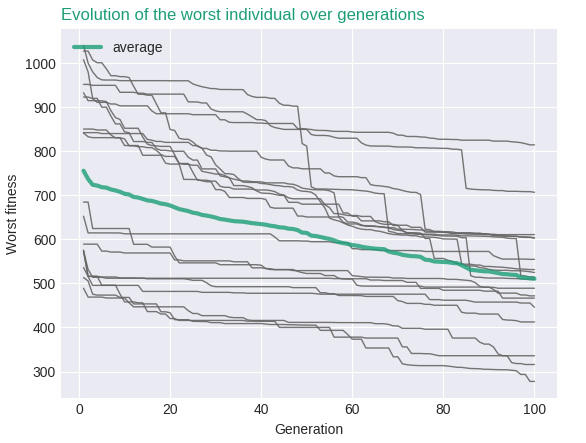
\includegraphics[scale=0.55]{exp1_worstIndv.png}
	\caption{In grey, different executions of the first experiment 
	1}\label{f:grahp1}
\end{figure}

\subsection{Second Experiment}

Most executions from the previous experiment reached the maximum number of 
generations without stabilizing or converging. This means the EA may need a 
larger number of generations to fully evolve a solution. This is the hypothesis 
for the second experiment.


The set of operators is the same as the previous one. The parameters remain 
unchanged except for:
\begin{itemize}
	\item Number of generations: 1000
\end{itemize}
We also added two stop conditions: 10 generations without changes (stable 
population) or best fitness value below 0.01.


Although best levels obtained with this experiment are better than those 
evolved in the first experiment, the bad solutions have a really high fitness 
value. In table \ref{t:resOver}, we can see that average fitness of levels 
produced with this version of the EA is worse than the ones generated in the 
first experiment. It suggest that populations can be stuck for many generations 
before making any type of improvement. Any of the generated levels have a 
fitness below 0.01 or reached maximum number of generations, which means the 
termination criteria that stopped the evolution was that the population was 
stable, without any new individuals added for 10 generations. 
\begin{figure}[H]
	\centering
	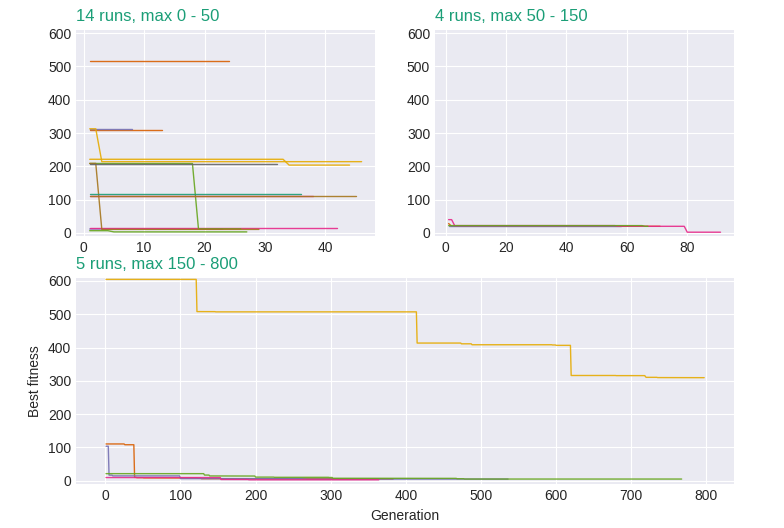
\includegraphics[scale=0.5]{exp2_explication.png}
	\caption{Best individual evolution for all executions, grouped by number of 
	generations}\label{f:grahp2}
\end{figure}
Figure \ref{f:grahp2} represents the evolution of the best individual of each 
execution. Most of them have no more than 50 generations, therefore the 
hypothesis for this experiment is not correct. Short evolutions show that the 
best individual at initialization is very similar to the last one. Slight 
improvements may be achieved by small mutations but it seems difficult for new 
generations to outperform previous ones. We can appreciate that significant 
improvements are most common in those executions with a poor initial 
population. Even the ones with several hundreds of generations struggle to 
improve the initial population.

\subsection{Third Experiment}
The previous experiment proved that the problem is not with the number of 
generations. Then it is more likely that there this EA is biased towards 
exploration rather than exploitation. The genetic operators are failing to 
create new individuals that inherit good traits from their parents. A new 
crossover operator could shift the focus to exploitation.


For the third experiment, the change introduced is in the crossover operator 
used. It was described in section \ref{ga:cross2}. The rest of the operators as 
well as the termination criteria are kept the same. 


Table \ref{t:resOver} shows that the results have radically improved as the 
average fitness of the best solutions drops to $0.0015$, a decrease of almost 
100\%. Additionally, it took less generations in general to reach those 
results. However, executions took longer on average, which makes sense given 
that a greater number of individuals would have been simulated. The average 
fitness of the population and the worst individual have similar values now, 
which suggest that in most executions the population did converge.

The levels are stable and the blocks do not fall when loading the level, but 
they could arguably be considered structures, since most of them consist in a 
few blocks displayed on the floor. The average amount of blocks is $6.26$, 
which is really close to the minimum amount of blocks allowed. However, given 
the proposed fitness function, it is completely logical that the evolution 
leads to this kind of arrangements. The more objects placed on the level, the 
more likely the individual is to not meet the requirements imposed by the 
constraints. It also makes sense to place objects near the ground, instead of 
one on top of the other.

\subsection{Fourth Experiment}
The previous EA generates levels with a number of blocks that tends to the 
minimum of blocks allowed which is 5. Such a small number of elements does not 
create interesting structures. A higher number of blocks may lead to more 
appealing levels. We test this in the fourth experiment.


The only parameter that was changed for this experiment is the minimum number 
of blocks from 5 to 10. 


The first thing to notice in this experiments (Table \ref{t:resOver}) is the 
increase of the average execution time: it went from 1.76 hours in the third 
experiment to 5.03 hours in this one. The time spent running the simulation for 
each population in this experiments and in the previous one should be similar. 
However, the number of executions drastically increased too. There is no doubt 
that placing at least ten objects is more difficult than placing 5. The average 
best fitness value slightly rose, while the average and worst values are lower. 
This suggest that the latest generations of this EA are less diverse than those 
from the third experiment.

%************************************************



%%%%%%%%%%%%%%%%%%%%%%%%%%%%%  CONCLUSIONS  %%%%%%%%%%%%%%%%%%%%%%%%%%%%
%
\section{Conclusions and Future Work} 
\label{sec:conclusions}
\subsection{Conclusion}

Here, we briefly recap several aspects of the development of this project. 
First, we reviewed the context of the problem: PCG. In section \ref{sec:intro}, 
we looked at the main reasons for its existence: from replacing human 
creativity where it cannot reach (unlimited or personalized) to enhancing and 
speeding the creative process. In some cases, PCG can  be considered a kind of 
creative expression for itself. The technical background to approach the 
problem is discussed in section \ref{sec:soa}.


This project was developed with a set of objectives in mind: The first goal was to explore the expressiveness and variability of SBPCG with evolutionary techniques. Perhaps the level of achievement of this one is not as easily measurable as the other three. It could seem like this objective has not been fully accomplished: only one SBPCG method has been implemented and tested. However, it was not in the scope of the project to test SBPCG in general, but in this particular case, for this particular game. Considering this, the method studied was sufficiently general and flexible to draw some conclusions about the topic. SBPCG methods are a potential good solution to offline content generation but it requires a great amount of problem-specific knowledge. Like any other form of creative work, the biggest issue may be how to measure how good, creative or enjoyable is the piece. The more rules the author adds, expressiveness starts to get lost as the results are variations of the same idea. However, it is crystal clear, from the experiments run in this project, that a lack of knowledge will lead to unexpected and even disappointing outcomes.

The second objective, adapting the game to extract data from execution, was 
certainly achieved. It was also a basic requirement to proceed with the rest of 
them. The game does provide the data, as long as the input is correctly 
structured. Although the original intention was to make it available on Linux, 
currently it can only be executed with the desired behaviour on Windows. 
Another issue is that the simulation is not easily adaptable. If the fitness 
function of the EA is changed and needs data that is not included in the output 
right now, the game would have to be changed and compiled again.

Producing stable structures under gravity was the third objective, and can be 
considered half a victory. The levels generated in the last experiments were 
undeniably stable. Whether or not they can be considered structures, that is 
arguable. Again, the main issue is how we evaluate the levels. In fact this is 
a matter of how we define what an Angry Birds' level \textit{is} and if that 
definition matches the fitness function. A lot of elements were correct, but 
the definition was not complete.

This idea brings us to the last objective, that was not achieved. Without 
results that match the definition of an Angry Birds level, placing the 
remaining objects would not have made the level playable. The partial 
achievement of the third goal, blocked the fourth one as this objective was 
dependent on the third one.

To conclude on an optimistic tone, this work provides an interesting insight 
into the SBPCG, through the completion---and failure---of those four goals.

\subsection{Future work}

In order to improve the results of the method, different constraints could be 
expressed as multiple objectives. Overlapping blocks, velocity and height could 
be treated as minimization objectives.

If we pay attention at the stages of evolution in this project, there is also 
room for improvement in the genetic operators. For example, the initialization 
produces a small amount of valid individuals which suggested that an elitist 
strategy for selection would work best. However, new experiments will help to 
better balance exploration and exploitation. 

Once we had a generator that meets our expectations, performance could be 
enhanced by the analysis of the best set of initial parameters using Analysis 
of Variance (or ANOVA), as presented in \cite{estevez2017statistical}. 

Some options were discarded for time limitations, so these could be main areas 
of development. The chromosome representation using generative grammatical 
encoding\cite{hornby2001advantages}, although it would radically change the 
structure of the method, might ensure that generated levels are consistent. 
This would require carefully selection the operators that would be the building 
blocks of the generative grammar.

Another important issue that needs to be addressed is the time performance. 
Right now the simulation is the main bottleneck in the execution. One way to 
speed up the process can be \textit{cleaning} the current simulation, getting 
rid of any unnecessary asset while maintaining the bare minimum. However, this 
will not solve the problem, since the content generator will still need to 
launch an external executable.

The communication between the simulation and the content generator is through 
read and write operations on disk, instead of memory. This could be avoided if 
both tools were integrated in one. If we aim for an online automatic generator, 
the generator should be integrated in the game. However, if our goal is to 
generate levels for mixed authorship, as an assistance to developers, it may be 
a better idea to integrate the simulation in the generator. This could be done 
by approximating in-game physics with real physics, as described in 
\cite{blum1970stability}. 


%************************************************

\section*{Acknowledgements}
% This paper has been supported in part by
% \href{http://geneura.wordpress.com}{GeNeura Team}, 
% projects TIN2014-56494-C4-3-P (Spanish Ministry of Economy and
% Competitiveness) and DeepBio (TIN2017-85727-C4-2-P).
Acks taking\\
this much space.

\bibliographystyle{splncs03}
\bibliography{angrybirds}



\end{document}
